\subsection{Mixture model of gamma-ray sources and limits on DM annihilation}
\label{sec:halos:results}

\subsection{Model optimization}
\label{sec:model-opt}

Our general aim is to either detect a population of DM subhalos among the \Fermi-LAT unassociated sources or to put an upper limit on $\langle\sigma v\rangle$ for different DM masses. For a fixed DM mass and annihilation channel, we determine the best-fit cross section $\langle\sigma v\rangle^*$ (optimized simultaneously with the other parameters) by maximizing the full likelihood built from the model in eq.~(\ref{eq:mixture}), defined as:
\be
\label{eq:L}
\mathcal{L}(\langle\sigma v\rangle, \pi_k, \btheta_\textrm{cov}) = \prod_{i=1}^{N^\textrm{ROI}_\textrm{unas}} \tilde{p}_\textrm{unas}(\bx_i|\sigmav,\pi_k, \btheta_\textrm{cov};\mdm,\textrm{ch.}).
\ee

We maximize eq.~(\ref{eq:L}) with the Expectation-Maximization (EM) algorithm, which is efficient for the cases of probabilistic mixture models~\cite{10.1162/089976602753284446_Saerens}, see appendix~\ref{app:EM} for more details.
From the ML point of view our approach is a semi-supervised learning algorithm.

Indeed, in supervised learning the model is fixed by the training data (including the PDFs for the different classes), while in unsupervised learning, the model is determined solely based on target data.
In our case, we use the associated sources (training data) to determine PDFs of the two classes of associated sources (which is similar to supervised learning), but we further modify the PDFs to account for the possible dataset shift between training and target data and add a new class of sources (which is similar to unsupervised learning).


We optimize the likelihood for a set of DM mass values: $\mdm$ = 10, 30, 100, 300, 1000 GeV, and determine, for each $\mdm$, the upper bound on $\sigmav$ at 95\% confidence level (CL) by profiling the test-statistic 
\be
\textrm{TS}(\sigmav) = -2\ln \frac{\mathcal{L}(\sigmav)}
{\mathcal{L}_\textrm{max}}, 
\label{eq:halos:TS}
\ee
where $\mathcal{L}(\sigmav)$ is the likelihood optimized over the rest of parameters $\pi_k$ and $\btheta_\textrm{cov}$, and $\mathcal{L}_\textrm{max}=\mathcal{L}(\sigmav^*,\pi_k^*,\btheta_\textrm{cov}^*)$ is the value of the likelihood for the best-fit parameters. 
Following the Wilks' theorem, we assume that TS follows the $\chi^2$ distribution. 
We compute the upper bound on $\sigmav$ as the value corresponding to the 95\% coverage probability (one-sided), which for one degree of freedom corresponds to
TS = 3.84.

We maximize the likelihood of the model in eq.~(\ref{eq:L}) to determine the best-fit parameters.
At first, we fix the DM contribution to be zero and determine the best-fit model with the known astrophysical sources only.
For reference, we show the model for the associated sources (no fitting) in the left panel of figure~\ref{fig:mixtures} and the best-fit model for unassociated sources in the middle and right panels.
In these plots, we display the distributions evaluated in the analysis ROI for $\alpha$ and $\beta$ parameters integrating over the flux coordinate for visualization purposes. We decompose the mixture model of eq.~(\ref{eq:mixture}) and associate the blue color with the extragalactic component and the red color with the Galactic component, both respectively weighted by their prior weight $\pi_k$ to highlight their relative contribution. The intensity of the color bar corresponds to the value of the component likelihood weighted by the prior weight, $\pi_k p(x | k)$, and a darker, more intense color is associated with regions where there is a higher probability of observing a certain source class. We will follow this convention for all upcoming distribution plots.

We note that the extragalactic sources are dominated by AGNs, which usually have close to a power-law spectra (small $\beta$ values).
The Galactic sources often have curved spectra (large $\beta$ values).
The relative contribution of Galactic sources is larger for the unassociated sources compared to the associated ones (brighter red color in the right panel compared to the left panel in figure~\ref{fig:mixtures}).
The model on the middle and right panels of figure~\ref{fig:mixtures} is obtained by optimizing the prior and covariate shift parameters, $\pi_k$ and $\btheta_\textrm{cov}$.
We display the optimized Galactic and extragalactic components separately in figure~\ref{fig:unas_mixture_astro}.
The corresponding best-fit parameters $\pi_k$ (the class prevalence) are presented in table~\ref{tab:class_prevalence_astro}. 
As qualitatively discussed above, the expected contribution of Galactic sources to unassociated sources at high latitudes (29\%) is significantly larger than the fraction of associated Galactic sources (6\%) in the ROI.
The right panel of figure~\ref{fig:mixtures} also shows the model's predictions for class probabilities of unassociated sources. 
\new{
We compare the relative importance of prior and covariate shift parts of the model in appendix~\ref{app:prior_vs_cov}, where
we find that the prior shift plays a more important role than the covariate shift.
In particular, for the model without the DM component, we find that the prior shift is preferred at $7\sigma$ significance (for one additional degree of freedom) compared to a model without either prior or covariate shifts, while the model with the covariate shift is preferred at $4.5\sigma$ significance (with 6 additional degrees of freedom). The model with both prior and covariate shifts is preferred at $6.7\sigma$ significance (with 7 degrees of freedom), i.e., most of the improvement is, indeed, due to the prior shift.
}


\begin{figure}[t]
    \centering
    \resizebox{0.99\textwidth}{!}{
    \hspace{-3mm}
    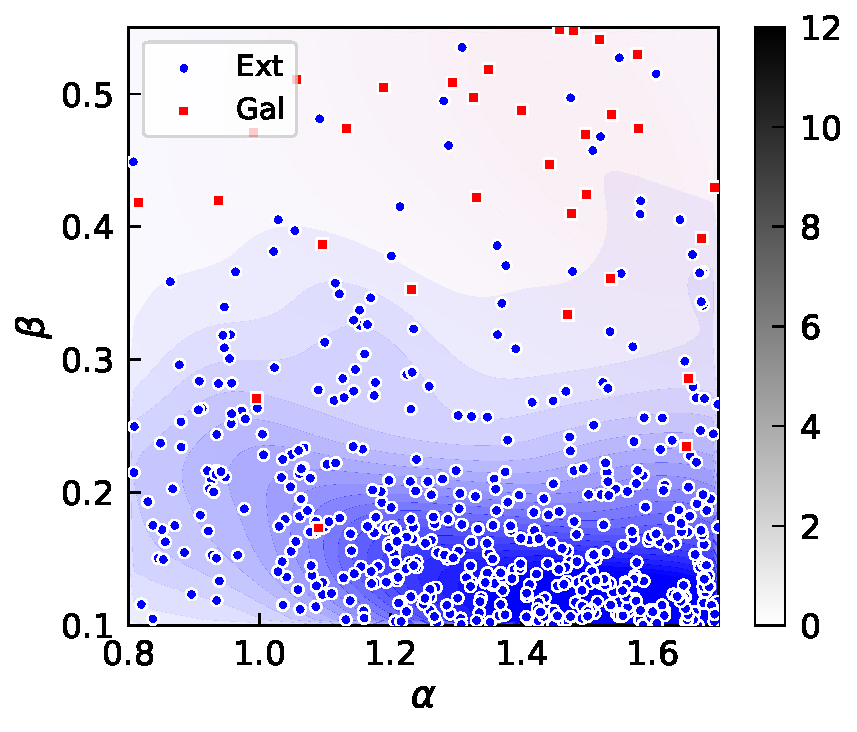
\includegraphics[width=0.33\linewidth]{sections/paper_dm_halos/img/model0/model0_as_sources_E0_1000MeV_labels.pdf}
    \hspace{-3mm}
    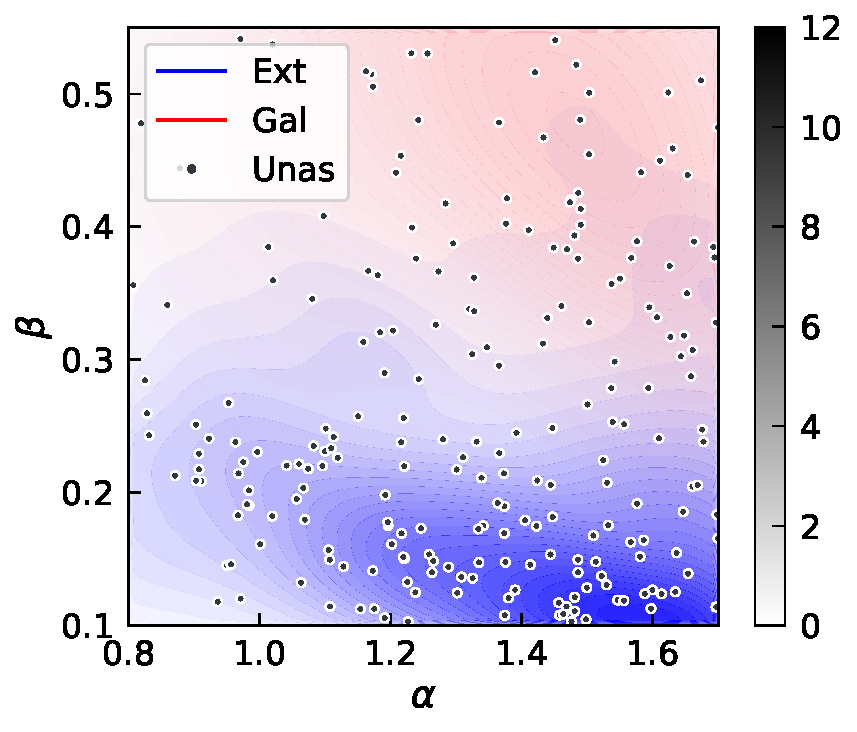
\includegraphics[width=0.33\linewidth]{sections/paper_dm_halos/img/model0/model0_covaraite_shift.pdf}
    \hspace{-3mm}
    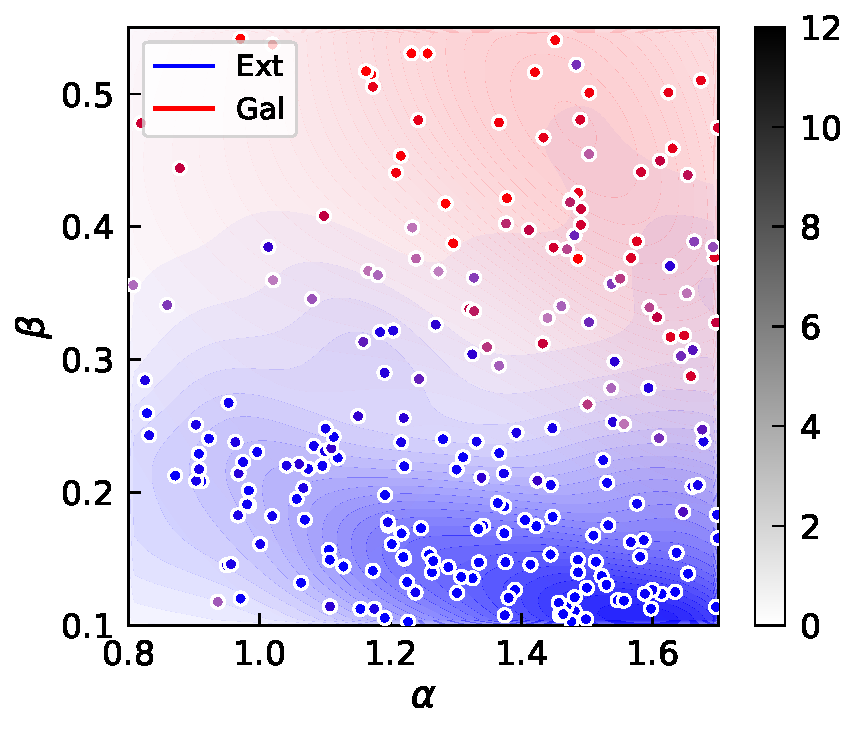
\includegraphics[width=0.33\linewidth]{sections/paper_dm_halos/img/predictions/model0_30GeV_prob_v4.pdf}
    }
    \caption{
    Distributions of sources in the plane of the spectral parameters ($\alpha$, $\beta$) for $E_0$ = 1~GeV.
    \panel{Left panel}: PDFs of Galactic and extragalactic sources weighted by the corresponding class fractions. The sources are colored according to the catalog class.
    \panel{Middle panel}: best-fit mixture model for the unassociated sources. The background colors show the individual components of the astrophysical-only model from eq.~(\ref{eq:mixture}), where the DM subhalo contribution is set to zero. Specifically, we plot the decomposition of the mixture model into class-conditional PDFs weighted by their best-fit class prevalence $\pi_k p(x | k)$ for the extragalactic (blue) and Galactic (red) populations. For visualization, the distributions are integrated over the flux dimension. The color bar represents the value of the resulting probability density (shown in gray to represent both red and blue colors).
    \panel{Right panel}: Class probabilities for unassociated 4FGL-DR4 sources (for $E_0 = 1 \, \textrm{GeV}$), on top of the mixture distribution (same as the middle panel). The color scale is proportional to the class probabilities, according to the formula $\textrm{color}(x_i)=\textrm{red}\cdot p(C_k= \textrm{gal}|x_i) + \textrm{blue}\cdot p(C_k=\textrm{ext}|x_i)$, e.g., a purple-colored source is a source for which the posterior class probabilities are similar and the classification is ambiguous. 
    }
    \label{fig:mixtures}
\end{figure}

\begin{figure}[t]
    \centering
    \resizebox{0.95\textwidth}{!}{
    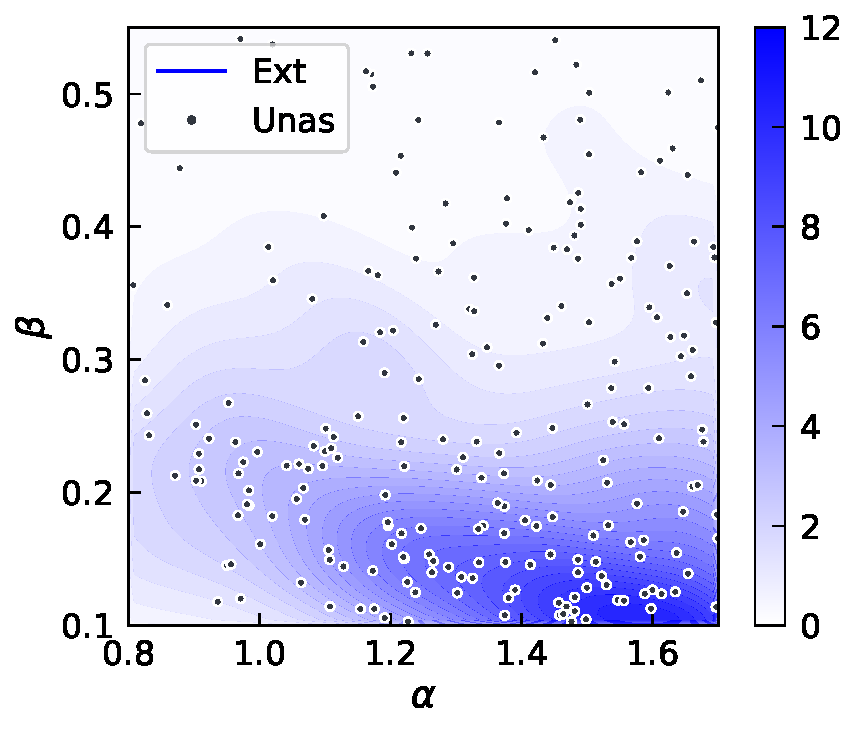
\includegraphics[width=0.49\linewidth]{sections/paper_dm_halos/img/model0/model0_covaraite_shift_ext.pdf}
    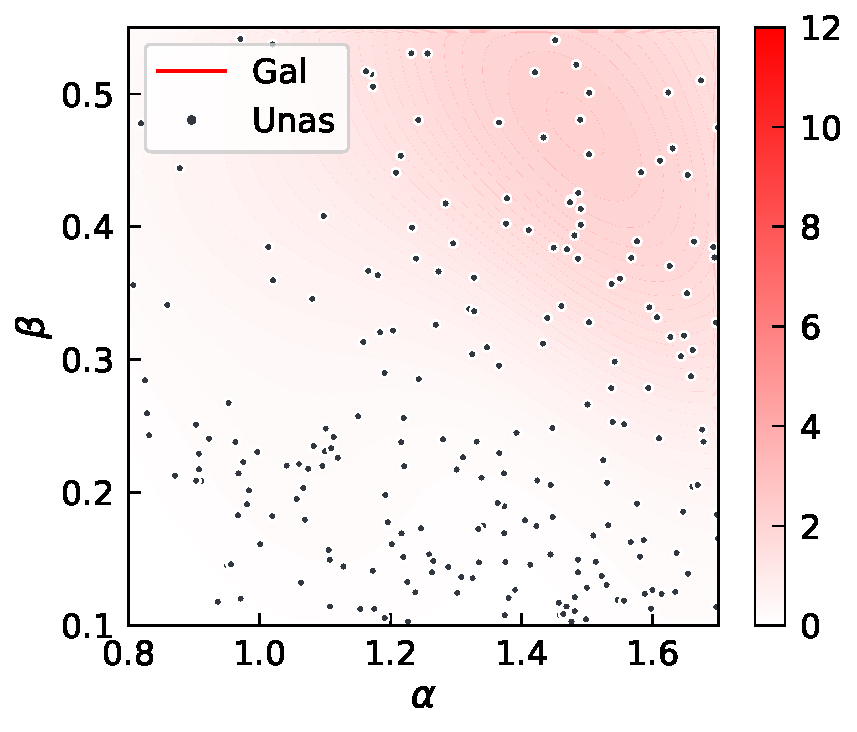
\includegraphics[width=0.49\linewidth]{sections/paper_dm_halos/img/model0/model0_covaraite_shift_gal.pdf}
    }
    \caption{Decomposition of the mixture model for unassociated sources with two classes (Galactic and extragalactic) for the ROI cut associated with $E_0 = 1$ GeV. The model is the same as in the middle and right panels of figure~\ref{fig:mixtures}.  
    \panel{Left panel}: extragalactic component. \panel{Right panel}: Galactic component.
    }
    \label{fig:unas_mixture_astro}
\end{figure}


\begin{table}[t]
\centering
% \resizebox{0.95\textwidth}{!}{
\begin{tabular}{|rccccc|}
%\multicolumn{6}{c}{\textbf{Best-fit astro-only model}} \\
\toprule
type & $N_{\textrm{ext}}$ & $N_{\textrm{Gal}}$ & \% Ext & \% Gal & $N_{\textrm{tot}}$\\
\midrule
assoc & 466 & 31 & 94\% & 6\% & 497\\
unas & 160.6 & 66.4 & 71\% & 29\% & 227\\
\bottomrule
\end{tabular}
\caption{Class prevalence for Galactic and extragalactic sources in the ROI. 
For the associated sources (second row) the numbers are derived from the 4FGL-DR4 catalog. 
For the unassociated sources (third row), the numbers correspond to the best-fit model with astrophysical components only (using $E_0 = 1$ GeV). 
The percent of galactic (\% Gal) and extragalactic (\% Ext) sources are given by the best-fit parameters $\pi_k$ in eq.~(\ref{eq:mixture}) for the two astrophysical components.
The expected number of Galactic and extragalactic sources among the unassociated ones is derived as $\pi_k \times N_\textrm{tot}$, where $N_\textrm{tot} = 227$ is the total number of unassociated sources in the ROI.
}
\label{tab:class_prevalence_astro}
\end{table}


\subsection{Dark matter limits}
\label{sec:dm-limits}

The best-fit model including the DM component with DM mass of 100 GeV and $\sigmav=3.4 \cdot 10^{-25} \textrm{cm}^3\textrm{s}^{-1}$ is shown in figure~\ref{fig:mixture_DM_tot}.
We simultaneously fit the parameters $\pi_k$, $\btheta_\textrm{cov}$ and $\sigmav$.
The corresponding components are presented in figure~\ref{fig:mixture_DM_components}.
The DM component is shown by the green color.%
\footnote{The class probabilities for unassociated sources in the astrophysical only model, as well as DM subhalo class probabilities for the different DM masses, are available online at \href{https://doi.org/10.5281/zenodo.17463823}{https://doi.org/10.5281/zenodo.17463823}.
}


Provided that all DM subhalos have the same gamma-ray spectra, the corresponding distribution of DM subhalos is much better localized in the $\alpha$ and $\beta$ plane than the extragalactic and Galactic components.
The spread in the DM subhalo distribution comes from statistical uncertainties in the reconstruction of spectral parameters.
We note that not only the overall normalization but also the shape of the distribution of DM subhalos in the right panel of figure~\ref{fig:mixture_DM_components}
changes for different annihilation cross sections and J-factor models (cf. figure~\ref{fig:DM_dist_countour}).
The reason is that the distribution depends on the relative contribution of subhalos with different J-factors, e.g., smaller J-factors correspond to proportionally smaller flux and larger uncertainties, which affect the shape of the distribution.
Nevertheless, for larger $\sigmav$ values the expected contribution of DM subhalos also increases. 


%%%%%% model with DM
\begin{figure}
    \centering
    %\resizebox{0.95\textwidth}{!}{
    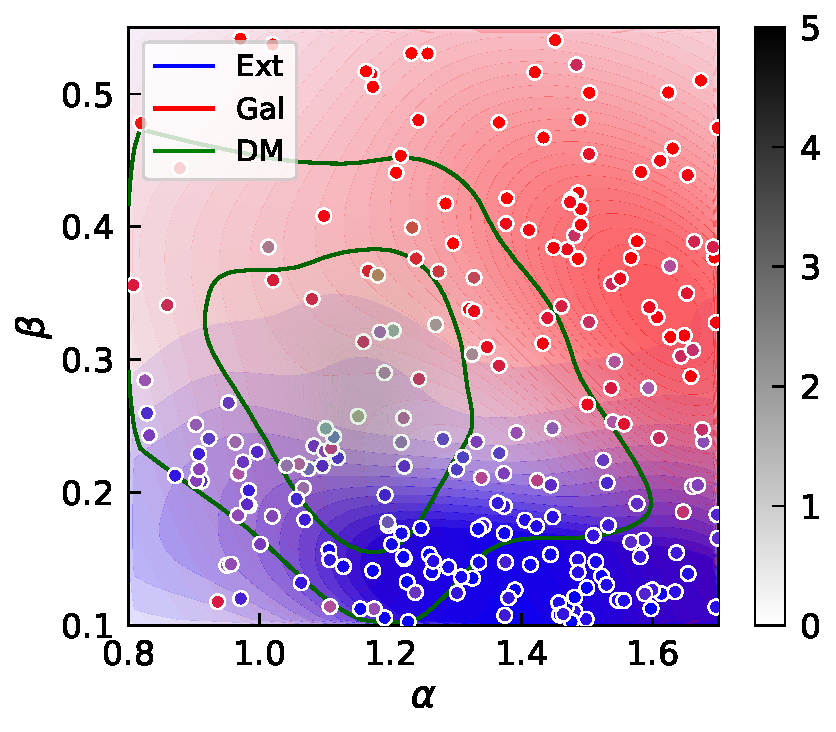
\includegraphics[width=0.49\linewidth]{sections/paper_dm_halos/img/predictions/best-fit_model_100GeV_posterior_prob.pdf}
    %}
    \caption{Mixture model for unassociated sources including the DM component with ${\mdm} = 100$ GeV, following the same conventions as in figure~\ref{fig:mixtures}.
    The green component represents the best-fit DM distribution for $\sigmav=3.4 \cdot 10^{-25} \textrm{cm}^3\textrm{s}^{-1}$. The green lines represent the 68\% and 95\% containment levels for the DM distribution.
    The background colors represent the class-conditional distributions weighted by their prior weight: $\pi_kp(x|k)$.
    Sources are colored according to their posterior class probability following the formula $\textrm{color}(x_i)=\textrm{red}\cdot p(C_k= \textrm{gal}|x_i) + \textrm{blue}\cdot p(C_k=\textrm{ext}|x_i) + \textrm{green}\cdot p(C_k=\textrm{DM}|x_i)$.
    }


    \label{fig:mixture_DM_tot}
\end{figure}

\begin{figure}
    \centering
    \resizebox{0.99\textwidth}{!}{
    \hspace{-3mm}
    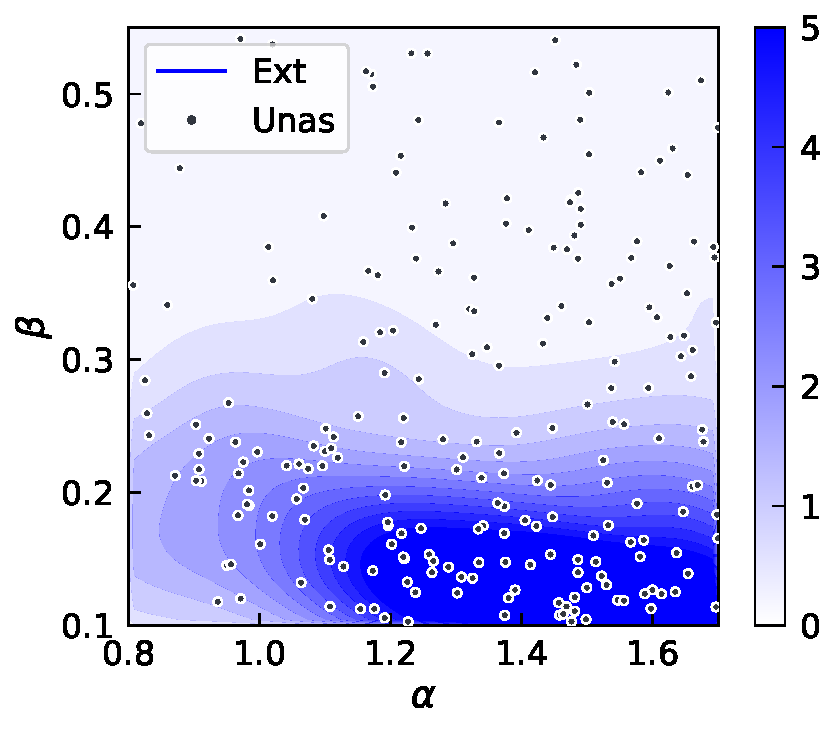
\includegraphics[width=0.32\linewidth]{sections/paper_dm_halos/img/mixture_with_dm/ext.pdf}
    \hspace{-3mm}
    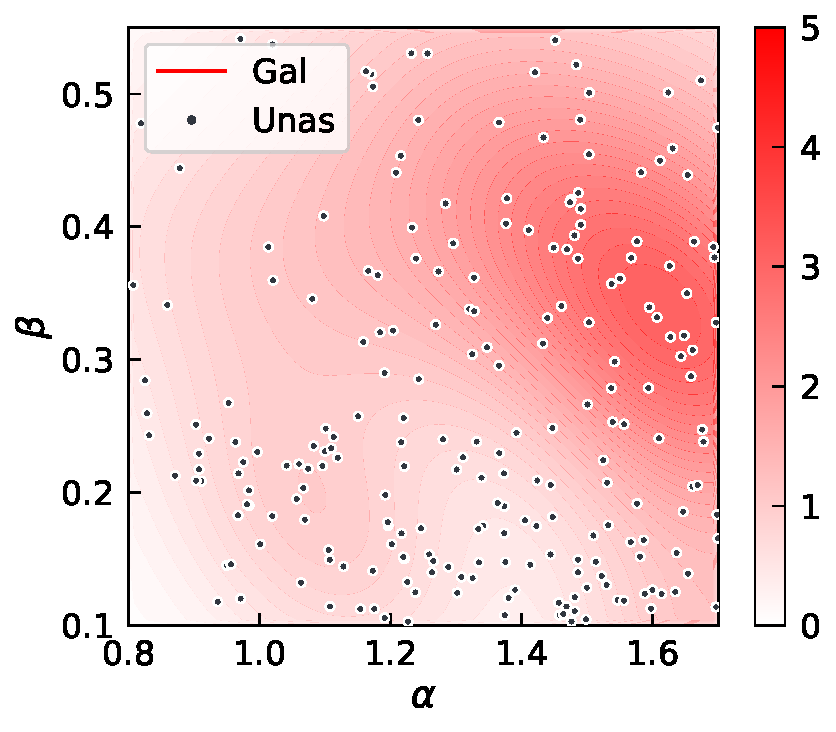
\includegraphics[width=0.32\linewidth]{sections/paper_dm_halos/img/mixture_with_dm/gal.pdf}
    \hspace{-3mm}
    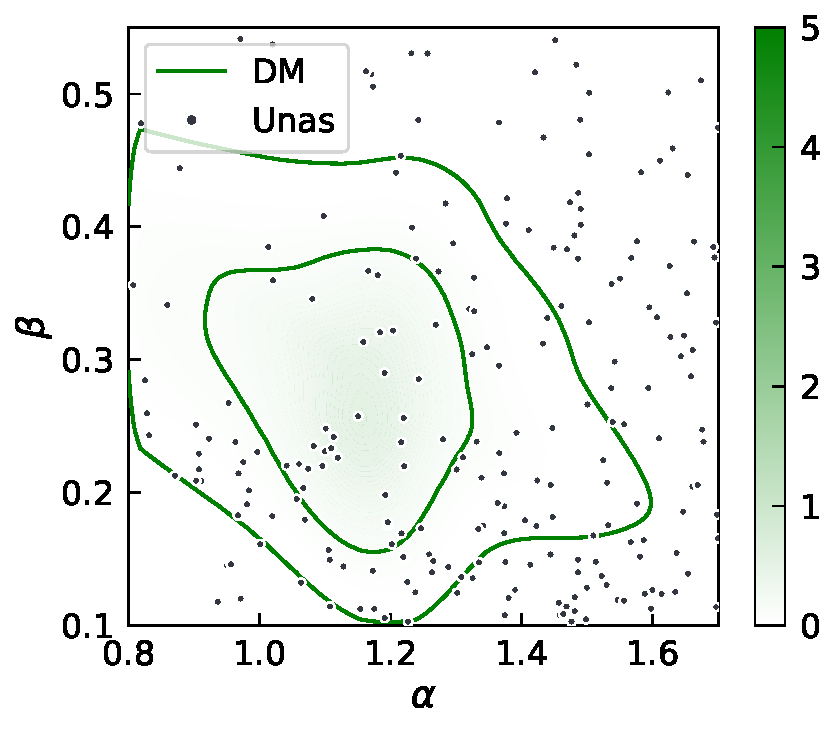
\includegraphics[width=0.32\linewidth]{sections/paper_dm_halos/img/mixture_with_dm/dm.pdf}
    }
    \caption{Components of the mixture model in figure~\ref{fig:mixture_DM_tot}, following the same conventions as in figure~\ref{fig:mixtures}.
    }
    \label{fig:mixture_DM_components}
\end{figure}


%%%% new position

We present the details of the best-fit model for the DM subhalo component (including upper limits in the annihilation cross section)
in table~\ref{tab:Nsub_values}.
Columns 2 to 6 show the best-fit model, e.g., the best-fit DM subhalo prevalence, the expected number of subhalos within our region of interest ($N_\textrm{subhalo}^\textrm{ROI}$) and for the full range of parameters ($N_\textrm{sub}^\textrm{total}$), as well as the best-fit thermally-averaged annihilation cross-section ($\sigmav$). The value of $\Delta \textrm{TS}_0 = -2(\log\mathcal{L}_0 - \log\mathcal{L}_\textrm{max})$ quantifies the preference for the best-fit model over a baseline astrophysical-only scenario. 
For all tested models, the significance is less than 2 sigma.
We notice that the largest possible contribution from DM subhalos is for $\mdm = 30$ GeV (although still not significant). 
\new{The expected number of DM subhalos of 15.4 for this DM mass  in our ROI is comparable, e.g., to 16 DM subhalo candidates reported in ref.~\cite{2019JCAP...07..020C}.
This comparison should be taken with a grain of salt, as the calculation in ref.~\cite{2019JCAP...07..020C} was performed for the 3FGL catalog (8 years of data) compared to the 4FGL-DR4 catalog (14 years of data) in our work with the J-factors based on the mass estimate within the tidal radius (cf. $J_\textrm{tidal}^{\Msub}$ in Section~\ref{sec:sim-jfactor}) compared to the J-factor integrated within $0.1^\circ$ from the center base on the maxima velocity used in table~\ref{tab:Nsub_values}.
}
\old{In this case} \new{We also notice that for $\mdm = 30$~GeV},  the expected contribution from Galactic sources (mostly millisecond pulsars) is the smallest.
This is to be expected, since the spectrum of DM annihilation in the $b\bar{b}$ channel is similar to the spectra of pulsars at this DM mass.
As a result, there may be a degeneracy between the DM subhalos and Galactic sources for this DM mass.
Provided that we do not find significant evidence for a signal from DM, we proceed to set conservative upper bounds on $\sigmav$ shown in the ``upper bound" section of the table.

\new{
In order to estimate the overall goodness of fit of the model in eq.~(\ref{eq:mixture}) without DM to the data,
we compare in appendix~\ref{app:model_goodness} the log likelihood of the fit to the data with the distribution of log likelihood values for the data generated from the best-fit model.
We find that the deviation of the log likelihood for the real data is less than $2\sigma$ smaller than the mean log likelihood value for the simulated data, i.e., the deviation is consistent with statistical fluctuations within $2\sigma$.
We also perform DM injection tests in appendix~\ref{app:DM_injection}.
We find that our method can recover the DM signal within statistical fluctuations: for all DM masses the  $\sigmav$ value for the injected signal is within the 68\% containment of the recovered $\sigmav$ values around the median recovered $\sigmav$.
}
\new{In addition, we determine the precision-recall curves for the classification of individual DM subhalos for 1000 simulations with injected DM signal (in case of $\mdm = 30$~GeV) and evaluate the average precision of our model in appendix \ref{app:pr_curve}.}


\begin{table}[t]
\centering
\resizebox{0.95\textwidth}{!}{%
\begin{tabular}{|l|ccccc|ccc|}
%\begin{tabular}{l ccccc ccc}
\toprule
 & \multicolumn{5}{c|}{\textbf{best-fit model}} & \multicolumn{3}{c|}{\textbf{upper bound}} \\ 
 $\mdm$ & \% DM & $N_\textrm{subhalo}^\textrm{ROI}$  & $N_\textrm{subhalo}^\textrm{total}$ & $\langle \sigma v \rangle$ & $\Delta \textrm{TS}_0$ & $N_\textrm{subhalo}^\textrm{ROI}$ & $N_\textrm{subhalo}^\textrm{total}$ & $\langle \sigma v \rangle$ \\
  $\textrm{[GeV]}$ & & & & [$\textrm{cm}^3 \, \textrm{s}^{-1}$] & & & & [$\textrm{cm}^3 \, \textrm{s}^{-1}$] \\
\midrule
10 & 0.0 & 0.00 & 0.00 & 0.0 & 0.0 & 2.83& 6.56& $5.6 \times 10^{-26}$\\
30 & 6.8 & 15.37 & 36.23 & $2.7 \times 10^{-25}$& 3.5 & 27.30 & 64.20 & $3.6 \times 10^{-25}$\\
100 & 2.4 & 5.45 & 6.21 & $3.4 \times 10^{-25}$ & 1.2 & 19.36 & 21.86 & $5.9 \times 10^{-25}$\\
300 & 2.0 & 4.59 & 7.66 & $1.1 \times 10^{-24}$ & 1.1 & 13.23 & 21.46 & $1.7 \times 10^{-24}$\\
1000 & 0.0 & 0.00 & 0.00 & 0.0 & 0.0 & 3.37& 13.75& $4.7 \times 10^{-24}$ \\
\bottomrule
\end{tabular}%
}
\caption{
Expected number of DM subhalos ($N_\textrm{sub}$) for the \textbf{best-fit model} and for the \textbf{95\% confidence upper bound} on the annihilation cross-section ($\sigmav$). In both cases, we report the subhalo count within our ROI and the total count. The test statistic difference quantifies the significance of the best-fit model over an astrophysical-only model, $\Delta \textrm{TS}_0 = -2(\log\mathcal{L}_0 - \log\mathcal{L}_\textrm{max})$. The number of subhalos, $N_\textrm{sub}$, is constrained to be non-negative.
}
\label{tab:Nsub_values}
\end{table}

%
%%%%%% bounds
\begin{figure}
    \centering
    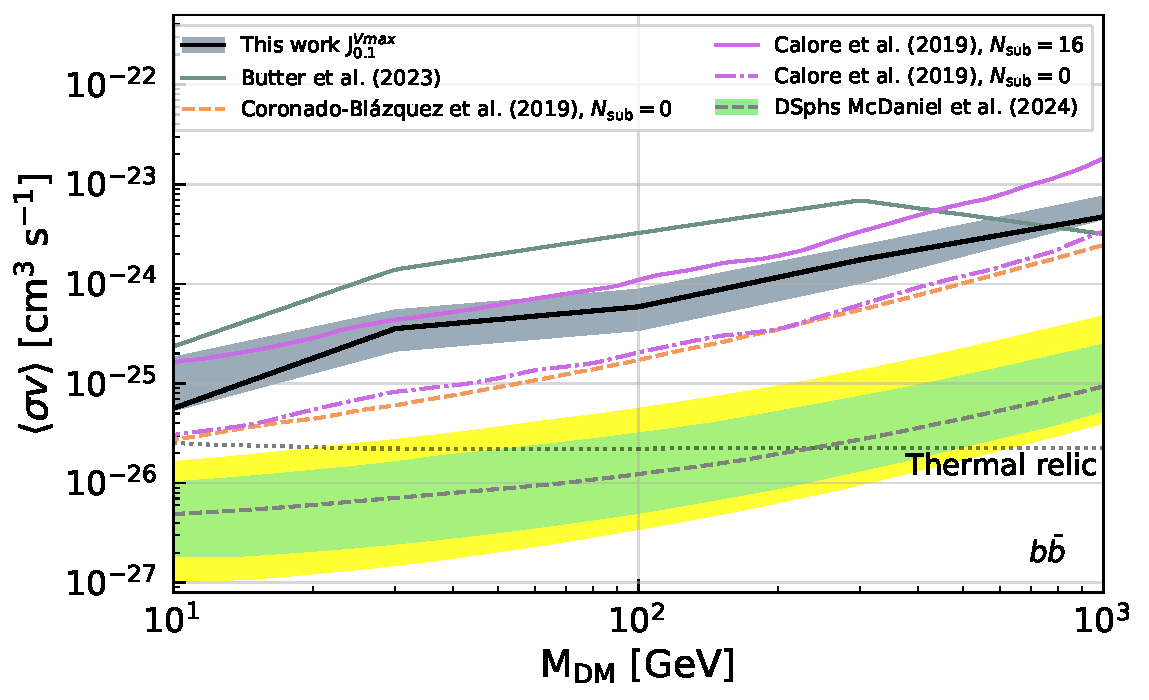
\includegraphics[width=0.80\linewidth]{sections/paper_dm_halos/img/bounds/sigmav_bounds_flux_bb_left.pdf}
    %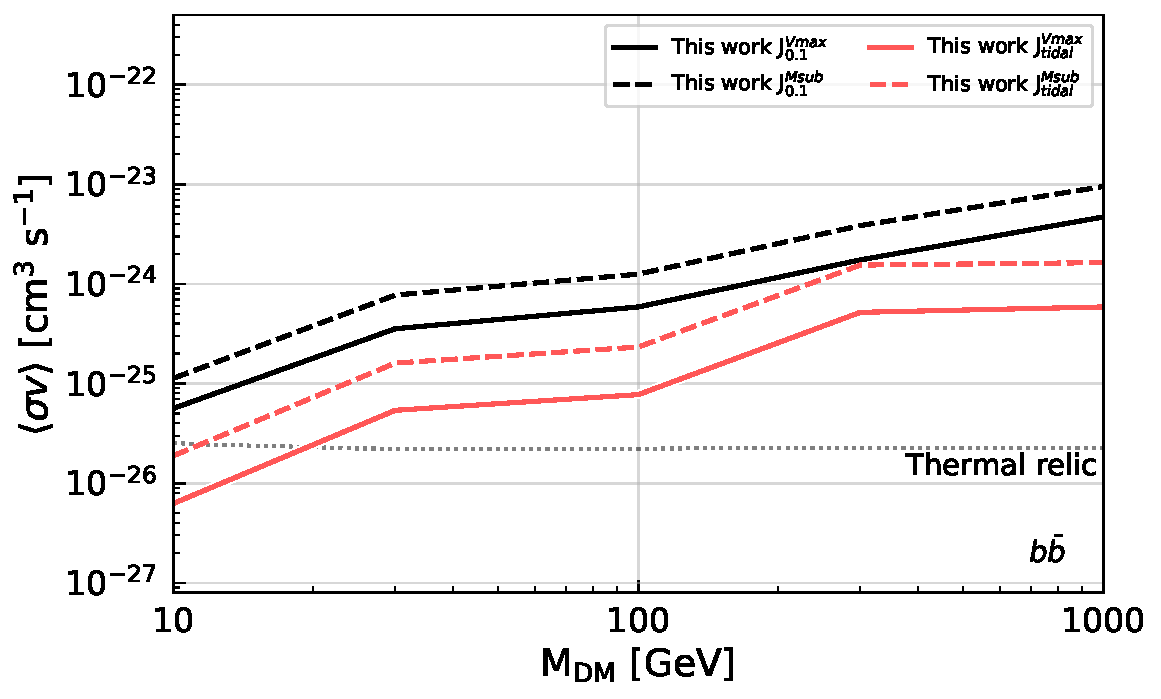
\includegraphics[width=0.70\linewidth]{sections/paper_dm_halos/img/bounds/sigmav_bounds_flux_bb_right.pdf}
    \caption{
    Upper bounds with 95\% confidence on the DM annihilation cross section $\sigmav$ in the $b\bar{b}$ channel. 
    %\newline
    %{Upper panel:} Comparison of our baseline results with literature. 
    Solid black line: our baseline limits derived with the 
    $V_\textrm{max}$ determination of the J-factor integrated within the radius of $0.1^\circ$.
    Gray band: 95\% containment of the upper limit due to statistical fluctuations of the distribution of sources.
    Solid and dashed purple lines: the limits derived by Calore et al. (figure 6 left panel%, turquoise and purple lines
    )~\cite{2019Galax...7...90C}. 
    Dashed orange line: limits derived by Coronado-Bl{\'a}zquez et al. (figure 5 upper panel%, black line
    )~\cite{2019JCAP...11..045C}. 
    Solid green line: the limits derived by Butter et al. (figure 11% solid green line
    )~\cite{2023JCAP...07..033B}.
    Green and yellow bands with dashed gray line: limits derived for dwarf spheroidal Galaxies at 68\% and 95\% confidence level by McDaniel et al. (figure 6 top left panel)~\cite{2024PhRvD.109f3024M}.
    Dotted black line: the expectation for the WIMP DM thermal relic cross-section from ref.~\cite{Steigman_2012}.
    }
    \label{fig:bounds-bb}
\end{figure}


\begin{figure}
    \centering
    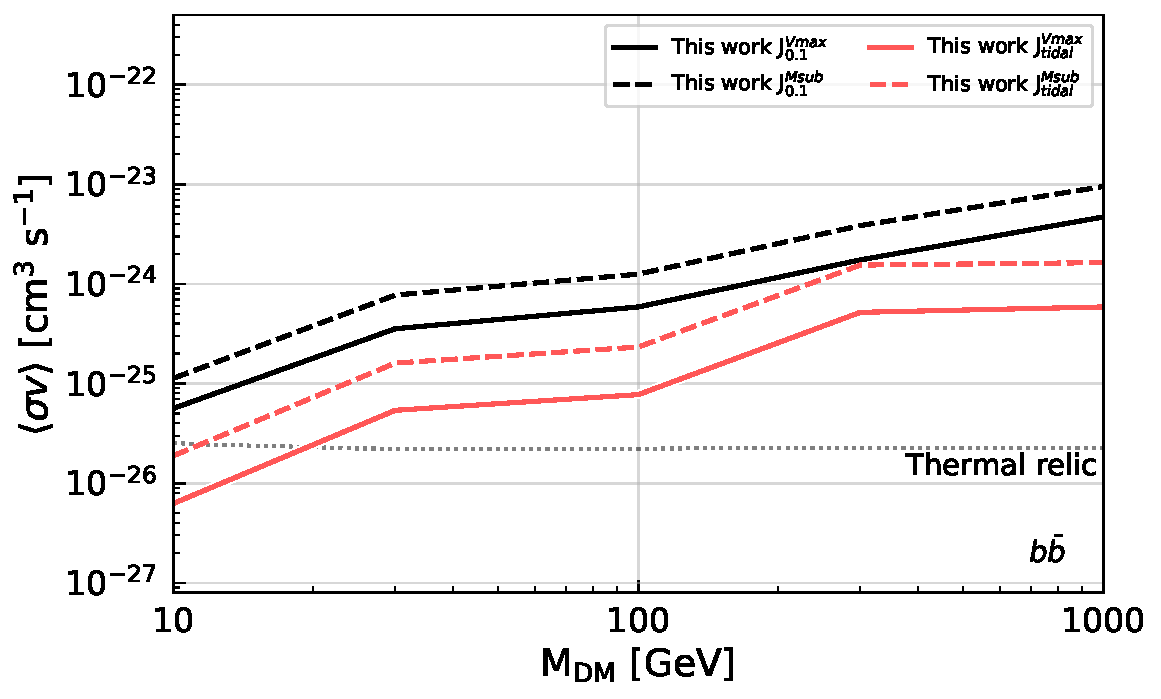
\includegraphics[width=0.80\linewidth]{sections/paper_dm_halos/img/bounds/sigmav_bounds_flux_bb_right.pdf}
    \caption{
    Comparison of the 95\% upper bounds on $\sigmav$ derived in this work for different choices of the J-factor.
    Solid (dashed) black line: the limit derived with the 
    $V_\textrm{max}$ ($M_\textrm{sub}$) determination of the J-factor integrated within the radius of $0.1^\circ$.
    Solid (dashed) red line: the limit derived with the 
    $V_\textrm{max}$ ($M_\textrm{sub}$) determination of the J-factor integrated within the tidal radius. 
    The uncertainty bands for the different J-factor models are proportional to the uncertainty band for our baseline model, $J_{0.1}^{Vmax}$ (figure~\ref{fig:bounds-bb}), with the same scaling factors as the ratios of the corresponding upper limits. These uncertainty bands are not plotted for clarity of presentation.
    }
    \label{fig:bounds-bb-J}
\end{figure}

We show the upper bounds on $\sigmav$ in figure~\ref{fig:bounds-bb}.
\old{where we also compare with the limits
obtained previous works.}
\old{To derive} The uncertainty band for the annihilation cross-section bound \new{is derived with} \old{we adopt} a bootstrap strategy. 
We identify the best-fit model for each DM mass and  use the probability density function for that model (cf. eq.~(\ref{eq:mixture})) to sample 100 new datasets via Hybrid (a.k.a. ``Hamilton'') Monte Carlo (HMC) \cite{2017arXiv170102434B} and the NUTS algorithm \cite{2011arXiv1111.4246H}. 
%%%%%
\new{For each simulated dataset, we derive the bounds on $\langle \sigma v \rangle$ and determine the $95\%$ containment interval for the resulting distribution of values. We further adjust the upper limit of this interval to conservatively account for potential systematic uncertainties associated with the presence of 4FGL sources, as detailed in Appendix~\ref{app:sim-ps}. This uncertainty range is represented by the gray shaded band in figure~\ref{fig:bounds-bb}.}
%%%%
For comparison we show the limit obtained by assuming that there are 16 DM subhalos in the 3FGL catalog by the purple solid line~\cite{2019Galax...7...90C}.
\new{We notice that our limit for $\mdm = 30$~GeV is close to the limit derived in ref.~\cite{2019Galax...7...90C}, although the upper limit on the number of DM subhalos in our analysis (27.3) is larger than the number of DM subhalo candidates (16) assumed in~\cite{2019Galax...7...90C} following the analysis of ref.~\cite{2019JCAP...07..020C}.
Our limit is slightly better due to longer observation time (14 years vs 8 years), which results in better flux sensitivity.
For other DM masses, 
our limit is better than the limit reported in~\cite{2019Galax...7...90C} due to smaller upper limits on the number of DM subhalo candidates.}
\old{as well as the best possible sensitivity of the 3FGL catalog to DM subhalos (assuming that no unassociated sources correspond to DM subhalos) shown by purple dash dotted line and the orange dashed line.}
\new{All of these upper limits on DM subhalo candidates, on the other hand, are larger than 1. As a result, the constraints on the DM annihilation cross sections are worse than the best possible constraints corresponding to zero observed DM subhalos, shown by the purple dash-dotted line~\cite{2019Galax...7...90C} and the orange dashed line~\cite{2019JCAP...11..045C} in figure~\ref{fig:bounds-bb}.}
\old{The solid green line corresponds to more recent bounds derived using an ML approach [31].}
\new{
Our limits are also significantly better for most of DM masses than in ref.~\cite{2023JCAP...07..033B} due to the very conservative approach in estimating the number of DM subhalos adopted in ref.~\cite{2023JCAP...07..033B}, where the number of possible DM subhalo candidates, e.g., for $\mdm = 30$~GeV is estimated to be 281 in the most conservative scenario.}

\old{In dashed gray, we plot}
\new{Dashed gray line in figure~\ref{fig:bounds-bb} shows} a recent bound derived using dwarf spheroidal galaxies~\cite{2024PhRvD.109f3024M} with 68\% and 95\% confidence bands \new{shown by green and yellow areas respectively.}
We note that the constraints derived in this work are an order of magnitude less stringent than the limits derived using dwarf spheroidal galaxies (even if we consider J-factors integrated to tidal radius for the subhalos).
Provided that the values of J-factors $\lesssim 10^{20} \mathrm{GeV^2 cm^{-5}} $ for the brightest dwarf galaxies \citep{2024PhRvD.109f3024M} are comparable to the brightest subhalos (cf. figure~\ref{fig:Jfactors}), the main reason for the less stringent constraints is that the positions and J-factors of the dwarf galaxies are known (although with some uncertainties), while the subhalos can be at any position in the sky.

In figure~\ref{fig:bounds-bb-J}, we display a comparison of the upper bounds for different choices of the J-factor.
In particular, the limits for the J-factor integrated within $0.1^\circ$ for the $V_\textrm{max}$ and $M_\textrm{sub}$ J-factor
determination methods are shown by the black solid and dashed lines respectively. 
The limits corresponding to the J-factor integrated up to the tidal radius for 
the $V_\textrm{max}$ and $M_\textrm{sub}$ J-factor determination methods are shown by the red solid and dashed lines, respectively.



The limits presented in figures~\ref{fig:bounds-bb} and \ref{fig:bounds-bb-J} are derived assuming the velocity-independent DM annihilation cross section.
In case of velocity-dependent annihilation cross section, e.g., due to Sommerfeld enhancement \cite{2009PhRvD..79a5014A, Piccirillo:2022qet, Lacroix:2022cjm, Facchinetti:2022jtd}
the relative contribution of small subhalos close to the Earth, which have a smaller velocity dispersion than the dwarf galaxies, will be more important.
In particular, a significant population of subhalos at distances of a few kpc with typical velocity dispersion of a few km/s is expected \cite{2024MNRAS.530.2496A}.
These subhalos can have a factor of a few larger enhancement of annihilation cross section compared to the dwarf galaxies, where the typical velocity dispersion has a peak in the distribution around 10 km/s (e.g.,~\cite{2018JCAP...04..035L}).
The actual enhancement of the limits from subhalos compared to the dwarf galaxies depends on the details of the model (e.g., there should be no saturation of enhancement down to velocities of a few km/s), on the integral of the velocity dispersion for the subhalos, and on the relative contribution of small subhalos in the vicinity of the Earth and large distant subhalos.
This detailed analysis is differed to a future work.

